\documentclass[wide,a4paper,titlepage,12pt] {article}
\usepackage{polski}
\usepackage[UTF8]{inputenc}
\usepackage{listings}
\usepackage{slashbox}
\usepackage[table]{xcolor}
\usepackage{graphicx,pdflscape}
\usepackage{placeins}
\usepackage{reportshelper}
\usepackage{longtable}

\title{Schemat Aproksymacyjny dla $P_{2}||C_{max}$}
\author{Jacek Wieczorek (181043)}

% Title page layout (fold)
\makeatletter
\renewcommand{\maketitle}{
  \begin{titlepage}
    \begin{center}
      \vspace*{3cm}
      \LARGE \@title \par
      \vspace{2cm}
      \textit{\small Autorzy:}\par
      \normalsize \@author\par \normalsize
      \vspace{3cm}
      Prowadzący : mgr inż. Karolina Mokrzysz\\
      Poniedziałek TP 11.00 - 13.00\\
      \vspace{3cm}
      Wydział Elektroniki\\ III rok \par
      \vspace{3cm}
      \small \@date
    \end{center}
  \end{titlepage}
}
\makeatother

\begin{document}
  \maketitle
  \section{Opis problemu}
\paragraph{}
 Celem laboratorium jest zaimplementowanie algorytmu szeregowania $n$ zadań na $2$ równolegle działających procesorach -  $P_{2} || C_{max}$ za pomocą wielomianowego schematu aproksymacyjnego \textit{PTAS}.

\section{PTAS}
\paragraph{}
Wielomianowy schemat aproksymacji (ang. Polynomial-time approximation scheme, w skrócie PTAS) to algorytm aproksymacyjny, który pozwala na uzyskanie dowolnie dobrego rozwiązania przybliżonego danego problemu optymalizacyjnego, i którego złożoność czasowa jest wielomianowa dla każdej żądanej dokładności.

\paragraph{}
Algorytm $A$ jest wielomianowym schematem aproksymacji dla problemu $\Pi$ jeśli spełnione są następujące warunki:
\begin{itemize}
    \item dla każdego odpowiedniego $\varepsilon$ A jest algorytmem $\varepsilon$-aproksymacyjnym dla $\Pi$,
    \item dla każdego odpowiedniego $\varepsilon$ złożoność czasowa $A$ jest wielomianowa ze względu na rozmiar instancji problemu podanej na wejściu $A$.
\end{itemize}

\section{Opis algorytmu}
\paragraph{}
\begin{itemize}
  \item Krok 1 : Posortuj zadania malejąco wg czasu ich wykonania
  \item Krok 2 : Przyporządkuj $k$-pierwszych zadań w sposób optymalny
  \item Krok 3 : Pozostałe $n-k$ zadań przyporządkuj za pomocą algorytmu \textit{LPT} 
\end{itemize}

\section{Dowód wielomianowości}
\paragraph{}
\begin{itemize}
  \item Sortowanie: $O(nlogn)$
  \item Przyporządkowanie 1 : przegląd zupełny przy pomocą wektora binarnego - $2^k$
  \item Przyporządkowanie \textit{LPT} : $O(n-k)$
\end{itemize}

\paragraph{}
Złożóność obliczeniowa : $O(nlogn + 2^k)$
\paragraph{}
Dokładność : 
$\varepsilon = \frac{1}{1+\lfloor k/2 \rfloor}$
\paragraph{}
 Wynika z tego, iż k = $O(\frac{1}{\varepsilon})$
\paragraph{}
Co daje nam złożoność obliczeniową algorytmu : $O(nlogn + 2^{\frac{1}{\varepsilon}})$

\section{Implementacja}
\paragraph{}
\putcode{code/algo.cs}{java}

\section{Testy}
\paragraph{}
W celu przeprowadzenia dokłądnej analizy wykonanych zostało szereg testów badających czas wykonania algorytmu w zależności od parametru $n$ i $\varepsilon$. W przypadku badania czasu wykonania kazdej instancji wykonano po 3 testy, a prezentowany wynik jest ich średnią arytmetyczną. Mimo iż program posiada graficzny interfejs użytkownika, moduł testowy wykonany został jako aplikacja konsolowa.

\paragraph{}

\begin{center}
  \begin{longtable}{|c|c|c|}
    \hline
    n & $\varepsilon$ & time[ms]\\ \hline
    100 & 0,5&  0 \\ \hline
    100 & 0,45 & 0\\ \hline
    100 & 0,4 & 0\\ \hline
    100 & 0,35 & 0\\ \hline
    100 & 0,3 & 0\\ \hline
    100 & 0,25 & 0\\ \hline
    100 & 0,2 & 0\\ \hline
    100 & 0,15 & 0\\ \hline
    100 & 0,1 & 0\\ \hline
    100 & 0,05 & 126\\ \hline
    5100 & 0,5 & 243,333\\ \hline
    5100 & 0,45 & 243\\ \hline
    5100 & 0,4 & 243\\ \hline
    5100 & 0,35 & 242,333\\ \hline
    5100 & 0,3 & 242\\ \hline
    5100 & 0,25 & 242,333\\ \hline
    5100 & 0,2 & 243\\ \hline
    5100 & 0,15 & 242\\ \hline
    5100 & 0,1 & 243\\ \hline
    5100 & 0,05 & 366\\ \hline
    10100 & 0,5 & 954,333\\ \hline
    10100 & 0,45 & 953,333\\ \hline
    10100 & 0,4 & 952,333\\ \hline
    10100 & 0,35 & 952\\ \hline
    10100 & 0,3 & 950,666\\ \hline
    10100 & 0,25 & 950,666\\ \hline
    10100 & 0,2 & 957,666\\ \hline
    10100 & 0,15 & 1038,33\\ \hline
    10100 & 0,1 & 952\\ \hline
    10100 & 0,05 & 1080\\ \hline
    15100 & 0,5 & 2149,66\\ \hline
    15100 & 0,45 & 2129\\ \hline
    15100 & 0,4 & 2128\\ \hline
    15100 & 0,35 & 2127,33\\ \hline
    15100 & 0,3 & 2125,33\\ \hline
    15100 & 0,25 & 2128\\ \hline
    15100 & 0,2 & 2129,33\\ \hline
    15100 & 0,15 & 2128,66\\ \hline
    15100 & 0,1 & 2328,33\\ \hline
    15100 & 0,05 & 2253\\ \hline
    20100 & 0,5 & 3769,66\\ \hline
    20100 & 0,45 & 3779,33\\ \hline
    20100 & 0,4 & 3769,66\\ \hline
    20100 & 0,35 & 3767,33\\ \hline
    20100 & 0,3 & 3766,33\\ \hline
    20100 & 0,25 & 3773\\ \hline
    20100 & 0,2 & 3774,66\\ \hline
    20100 & 0,15 & 3780\\ \hline
    20100 & 0,1 & 3776,33\\ \hline
    20100 & 0,05 & 3894,33\\ \hline
    25100 & 0,5 & 6131\\ \hline
    25100 & 0,45 & 6044,66\\ \hline
    25100 & 0,4 & 5898\\ \hline
    25100 & 0,35 & 5883\\ \hline
    25100 & 0,3 & 5900,66\\ \hline
    25100 & 0,25 & 5879,66\\ \hline
    25100 & 0,2 & 5877\\ \hline
    25100 & 0,15 & 5888\\ \hline
    25100 & 0,1 & 5886\\ \hline
    25100 & 0,05 & 6003,66\\ \hline
    \caption{Wynik zależny od $\varepsilon$ i $n$}\\


  \end{longtable}
\end{center}

\putpicturescale{img/wyk1.PNG}{Wykres zależności czasu od $\varepsilon$}{1.0}{}
\newpage
\putpicturescale{img/wyk2.PNG}{Wykres zależności czasu od $n$}{1.0}{}

\paragraph{} % (fold)
Analizując powyższe dane można wywnioskować, iż największy wpływ na czas wykonywania algorytmu ma rozmiar instancji problemu $n$. Na Rysunku 1 przedstwiono zależność pomiędzy czasem wykonania algorytmu, a wartością $\varepsilon$ dla instancji o stałym rozmiarze $n$. Wykres obu funkcji przez dłuższy okres jest linią poziomą, dopiero dla ostaniego parametru nieznacznie wzrasta,lecz wciąż liniowo. Dla wartości parametru $\varepsilon = 0.05$ długość problemu, którą należy uszeregować dokładnie wzrasta znaczniej, niż w poprzednich przykładach. Z powodu zbyt długiego czasu wykonywania, nie przeprowdzone zostały testy dla $\varepsilon = 0.01$.

\paragraph{}
Analizując wykres przedstawiony na Rysunku 2 można dojść do wniosku, iż bez znaczącej zmiany parametru $\varepsilon$ np. 0.01 czas wykonywania algorytmu dla tych samych instancji problemu, ale większych parametrach $\varepsilon$ jest bardzo zbliżony.   

\section{Wnioski}
Algorytm \textit{PTAS} jest jednym z łatwiejszych algorytmów obliczania przyblliżonej wartości dla skomplikowanych problemów \textit{NPh i sNPh}. Jednak by uzyskać wyniki z zadowalającą dokładnością, należy użyć małych parametrów $\varepsilon$, co wiąże się z dużym nakładem czasu na obliczanie dokładnych wyników i zbliża algorytm do przeglądu zupełnego (w tym przypadku).

\paragraph{}
Głównym obszarem zastosowań algorytmu \textit{PTAS} są sytuacje, gdy możemy sobie pozwolić na dość duży błąd rozwiązania. 
\end{document}



% \begin{figure}[htbp]
 %     \begin{center}
  %      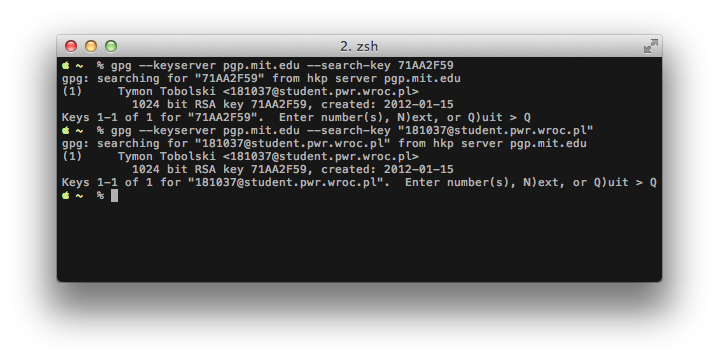
\includegraphics[scale=0.5]{screen/11.png}
   %     \caption{}
    %  \end{center}
    %\end{figure}